\documentclass[a4paper,14pt]{extreport}
  \usepackage[left=1.5cm,right=1.5cm,
      top=1.5cm,bottom=2cm,bindingoffset=0cm]{geometry}
  \usepackage{scrextend}
  \usepackage[T1,T2A]{fontenc}
  \usepackage[utf8]{inputenc}
  \usepackage[english,russian,ukrainian]{babel}
  \usepackage{tabularx}
  \linespread{1.5}
  \usepackage{amssymb}
  \usepackage{color}
  \usepackage{amsmath}
  \usepackage{mathrsfs}
  \usepackage{listings}
  \usepackage{graphicx}
  \graphicspath{ {./images/} }
  \usepackage{lipsum}
  \usepackage{xcolor}
  \usepackage{hyperref}
  \usepackage{tcolorbox}
  \usepackage{tikz}
  \usepackage[framemethod=TikZ]{mdframed}
  \usepackage{wrapfig,boxedminipage,lipsum}
  \mdfdefinestyle{MyFrame}{%
  linecolor=blue,outerlinewidth=2pt,roundcorner=20pt,innertopmargin=\baselineskip,innerbottommargin=\baselineskip,innerrightmargin=20pt,innerleftmargin=20pt,backgroundcolor=gray!50!white}
   \usepackage{csvsimple}
   \usepackage{supertabular}
  \usepackage{pdflscape}
  \usepackage{fancyvrb}
  %\usepackage{comment}
  \definecolor{ggreen}{rgb}{0.4,1,0}
  \definecolor{rred}{rgb}{1,0.1,0.1}
  \usepackage{array,tabularx}
  \usepackage{colortbl}

  \usepackage{varwidth}
  \tcbuselibrary{skins}
  \usepackage{fancybox}

  \definecolor{ggreen}{rgb}{0.4,1,0}
  \definecolor{rred}{rgb}{1,0.1,0.1}
  \definecolor{amber}{rgb}{1.0, 0.75, 0.0}
  \definecolor{babyblue}{rgb}{0.54, 0.81, 0.94}
  \definecolor{asparagus}{rgb}{0.53, 0.66, 0.42}
  \definecolor{chartreuse}{rgb}{0.5, 1.0, 0.0}
  \definecolor{darkorchid}{rgb}{0.6, 0.2, 0.8}
  \usepackage{fp}

  \usepackage{float}
  \usepackage{wrapfig}
  \usepackage{framed}
  %for nice Code{
  \lstdefinestyle{customc}{
    belowcaptionskip=1\baselineskip,
    breaklines=true,
    frame=L,
    xleftmargin=\parindent,
    language=C,
    showstringspaces=false,
    basicstyle=\small\ttfamily,
    keywordstyle=\bfseries\color{green!40!black},
    commentstyle=\itshape\color{purple!40!black},
    identifierstyle=\color{blue},
    stringstyle=\color{orange},
  }
  \lstset{escapechar=@,style=customc}
%}


\begin{document}

\newtcbox{\xmybox}[1][red]{on line, arc=7pt,colback=#1!10!white,colframe=#1!50!black, before upper={\rule[3pt] {0pt}{10pt}},boxrule=1pt,boxsep=0pt,left=6pt, right=6pt,top=2pt,bottom=2pt}


\pagecolor{white}
\begin{titlepage}
    \begin{center}
      \large
      Національний технічний університет України \\ "Київський політехнічний інститут імені Ігоря Сікорського"


      Факультет Електроніки

      Кафедра мікроелектроніки
      \vfill

      \textsc{ЗВІТ}\\

      {\Large про виконання практичної роботи №4\\
        з дисципліни: «Твердотільна електроніка-2»\\[1cm]

        Передавальна характеристика інвертора

      }
    \bigskip
  \end{center}
  \vfill

  \newlength{\ML}
  \settowidth{\ML}{«\underline{\hspace{0.4cm}}» \underline{\hspace{2cm}}}
  \hfill
  \begin{minipage}{1\textwidth}
  Виконавець:\\
  Студент 3-го курсу \hspace{4cm} $\underset{\text{(підпис)}}{\underline{\hspace{0.2\textwidth}}}$  \hspace{1cm}Р.\,П.~Фіцай\\
  \vspace{1cm}

  Перевірив: \hspace{6.1cm} $\underset{\text{(підпис)}}{\underline{\hspace{0.2\textwidth}}}$  \hspace{1cm}Л.\,М.~Королевич\\

  \end{minipage}

  \vfill

  \begin{center}
  2021
  \end{center}
\end{titlepage}


\begin{center}ЗАВДАННЯ\end{center}

Розрахувати передавальні характеристики інвертора на МДН-транзисторах з 
індукованим каналом. Рухливість в каналі рівна 1/2 від об'ємної ружливості у довіднику. 
W/L=2 (нижній транзистор), W/L=1/2 (верхній транзистор)



\begin{figure}[h]
  \begin{center}
    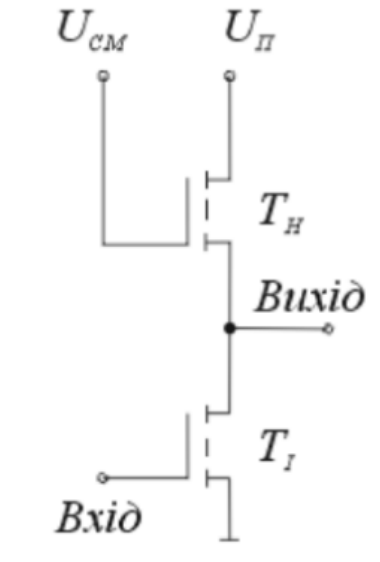
\includegraphics[width= 0.25\linewidth]{1.png}
  \end{center}
  \caption{Схема інвертора.}
\end{figure}

\begin{center}Виконання\end{center}

Знайдемо вираз, що описує круту ділянку передавальної характеристики:
$$
\begin{array}{c}
k_{L}\left[\left(U_{cm}-U_{\text {sux }}\right)-U_{\text {nop }}\right]^{2}=k_{I}\left(U_{\text {ax }}-U_{\text {nop }}\right)^{2} \\
U_{\text { см }}=E=11 B; \quad U_{\text {nop }}=1,6 B
\end{array}
$$


$$
\begin{array}{c}
U_{\text {Вux } 1}=\dfrac{-\left(2 U_{\text {nop }}-2 U_{\text {cм}}\right)+\sqrt{D}}{2}, \\
U_{\text {Вux } 1}=\dfrac{-\left(2 U_{\text {nop }}-2 U_{\text {cм}}\right)-\sqrt{D}}{2} .
\end{array}
$$

Знайдемо вираз, що описує пологу ділянку передавальної характеристики:
Виразивши $U_{\text {вих }}\left(\mathrm{U}_{\text{вх}}\right)$ отримаємо:
$$
U_{\text {вих1}}=\frac{\left(2 \frac{k_{L}}{k_{I}} U_{nop}-2 \frac{k_{L}}{k_{I}} U_{\text {см }}-2 U_{\text {вx }}+2 U_{\text {nоp }}\right)+\sqrt{D}}{2\left(\frac{k_{L}}{k_{I}}+1\right)}
$$


$$ U = U_{\text{см}} - U_{\text{пор}} = 9,4 $$











\end{document}
